%% This is free and unencumbered software released into the public domain.

%% Anyone is free to copy, modify, publish, use, compile, sell, or
%% distribute this software, either in source code form or as a compiled
%% binary, for any purpose, commercial or non-commercial, and by any
%% means.

%% In jurisdictions that recognize copyright laws, the author or authors
%% of this software dedicate any and all copyright interest in the
%% software to the public domain. We make this dedication for the benefit
%% of the public at large and to the detriment of our heirs and
%% successors. We intend this dedication to be an overt act of
%% relinquishment in perpetuity of all present and future rights to this
%% software under copyright law.

%% THE SOFTWARE IS PROVIDED "AS IS", WITHOUT WARRANTY OF ANY KIND,
%% EXPRESS OR IMPLIED, INCLUDING BUT NOT LIMITED TO THE WARRANTIES OF
%% MERCHANTABILITY, FITNESS FOR A PARTICULAR PURPOSE AND NONINFRINGEMENT.
%% IN NO EVENT SHALL THE AUTHORS BE LIABLE FOR ANY CLAIM, DAMAGES OR
%% OTHER LIABILITY, WHETHER IN AN ACTION OF CONTRACT, TORT OR OTHERWISE,
%% ARISING FROM, OUT OF OR IN CONNECTION WITH THE SOFTWARE OR THE USE OR
%% OTHER DEALINGS IN THE SOFTWARE.

%% For more information, please refer to <https://unlicense.org>
%%
\chapter{Introduction}
With the fast pace of today's market, the capability of the current silicon
technology, and the growing manufacturing costs of integrated circuits, it is
essential to develop digital circuits that meet the expected specifications at
the first releasing cycle.

The rapid development of silicon technologies seen from the 1960s to the early
2000s increased the integrated circuit's complexity and made their verification
process more challenging. Nowadays, silicon technology has reached an asymptotic
development curve, where lithography technologies are fighting against the law
of physics. Simultaneously, with the mobile and data-center revolution, the new
hardware market requirements have shifted from raw power to energy efficiency,
creating new design challenges.

To overcome these limitations, hardware designers started to incorporate more
and more hardware accelerators inside their designs to meet the required energy
efficiency without losing performances or relying on new silicon technologies.
This shift in hardware development presents new challenges for the verification
process. Each building block inside the new hardware needs to be verified
separately and collectively to ensure the final product's correct functionality.
As gate size decreases and the number of building blocks increases, the
verification process, while being essential to mitigate chips' respin, has
become one of the most significant NRE (Non-Recurring Engineering) costs for
chip manufacturers \cite{whydesingmustchange}.

Since the early 2000s, the industry has been researching and developing
verification tools to enhance verification engineers' productivity and shorten
the verification process. One of the main problems with the verification process
has been the barrier imposed by traditional hardware description languages like
VHDL or Verilog. Born almost four decades ago, these legacy HDLs lack the
reusability and extensibility features of modern languages, making it hard for
verification engineers to create the set of tools they needed. To overcome these
problems, in the early 2000s, companies and verification engineers started
developing and using other languages, like Spaceman e \cite{ieee-e2019} or
OpenVera \cite{openverapapaer} for verifying their designs.

In 2005, after many tentative approaches from the industry, IEEE standardized
(1800-2005) a new HDL called SystemVerilog that integrates verification
directives into the Verilog language to fill this gap between the verification
and the design process. SystemVerilog is an extension of the Verilog language
that introduced object-oriented concepts to the hardware world in order to
provide, to the language, the extensibility and reusability required in the
verification environment. SystemVerilog maintains the supports of behavioral,
register transfer level, and gate-level descriptions of Verilog while
introducing concepts like classes, a better type system, inheritances, cover
groups, assertions, and constrained random constructs, which focus solely on the
verification process \cite{sutherland2003overview}.


While SystemVerilog expanded hardware description languages' capabilities for
the verification process, it fell shortly on the needs of new hardware
designers' expectations. With the increasing number of different hardware
accelerators present in today's chip, the somewhat still limited capabilities of
the new type system are not suitable for quickly exploring the architectural
design space, or powerful enough for generic hardware parameterization. This is
extremely important because, to maximize the non-returning engineering costs,
hardware designers need to create hardware generators that can parametrically
generate different hardware configuration types for specific targets
\cite{whydesingmustchange}.

Even before SystemVerilog, designers started developing new ways to overcome the
conventional hardware description languages' limitations to fulfill their needs
to quickly explore new microarchitectures. One of their first approaches was to
use a companion language to preprocess macros for an underlying HDL language
\cite{bachrach2012chisel}. This approach enables a higher degree of flexibility
for creating hardware generators with the cost of losing the type system of the
underlying HDL and reducing the project's re-usability and maintainability. A
second approach was to create a Domain Specific Language (DSL) with a type
system aware of hardware constructors and defined on top of another programming
language. Usually, the donor language is a modern programming language with a
flexible type system allowing greater flexibility in parametrization. This
second approach, used by different languages \cite{bachrach2012chisel,
  github:kratos, github:hwt} has the benefit of allowing the hardware designer
to use all the tools and libraries available for the hosting language while
enforcing the design correctness with the type system.

One of these domain-specific languages is Chisel, a HDL based on the Scala
programming language. As a domain-specific language, Chisel can leverage the
Scala ecosystem of libraries and tools while also providing constructs to
accurately specify low-level hardware blocks. Currently, Chisel as a hardware
design platform overcomes SystemVerilog's limitation in component modularization
but lacks reliable verification primitives. One of the most critical primitives
offered by SystemVerilog is the possibility of defining Constrained Random
Stimuli. The generation of such stimuli is called Constrained Random
Verification (CRV), and this thesis describes the effort of implementing this
verification technique in Chisel. The fundamental of CRV is the automatic
creation and application of input stimuli to the hardware model, which are the
solutions of a satisfaction problem limited by a group of constraints. The
benefit of CRV is the possibility of automatically generating valid sequences of
input vectors without the manual intervention of the verification engineer. A
side effect of this technique is the generation of random stimuli that more than
not, trigger scenarios not envisioned by the verification engineers leading to a
fast discovery of bugs during the early stage of development.

This thesis describes the effort and the implementation of Constraint Random
Verification inside Chisel. The first part of the thesis introduces the
state-of-the-art tools available today for verification engineers and hardware
designers. The second part describes what functional verification is, why
constrained random verification is necessary, and the requirements for
integrating random constraint verification into Chisel. The third part describes
F-CSP, the first tentative attempt at integrating a constraint language into
Chisel. Lastly, the final part introduces Chisel-CRV, a constraint language part
of ``chiselverify" \cite{github:chiselverify}. Chiselverify is a library
developed as a research project conducted by the Embedded Systems research group
at the Technical University of Denmark, aiming to develop a Chisel library for
functional verification.


\section{Motivations}
Nowadays, the verification process for a new hardware design, is one of the
leading non-returning engineering costs that companies have to face before
launching a new product. This costly and time-consuming process is bounded by
the current verification tools available to the verification engineers. Today
the leading technologies for functional hardware verification are SystemVerilog
and UVM. Even though UVM and SystemVerilog are used by most of the industry,
these tools require a steep learning curve, proprietary simulators, and several
hundred lines of code, even for the verification of simple models. For a quick
comparison, picture \ref{fig:languagecomplexity} shows the number of
specification pages and keywords for different types of languages. SystemVerilog
has approximately eight times the number of keywords and specifications pages of
Scala. The only possible solution for increasing verification engineers'
productivity and accelerating the verification process is to make better
verification tools that integrate with hardware designers' development
environment. Comparably, SystemVerilog itself is not a monolithic language
\cite{mehta2018asic}, but instead a composition of four different languages,
describing constraints, assertions, and functional coverage. It is believed that
a similar approach can be applied to Chisel. Integrating verification directives
in Chisel will allow hardware designers and verification engineers to share the
same development environment where tools and utilities can be easily integrated
and shared across the team.



\section{Context}
This master thesis was carried out as part of the Master’s Degree in computer
science and engineering at the DTU. The project was developed within the DTU
project context with digital design verification and validation, which is
focused on researching novel methods and technologies in functional verification
of digital designs.

\begin{itemize}
    \item The author of this document: \thesisauthor
    \item Faculty supervisor: \thesissupervisor
\end{itemize}

\begin{figure}[!h]
\centering
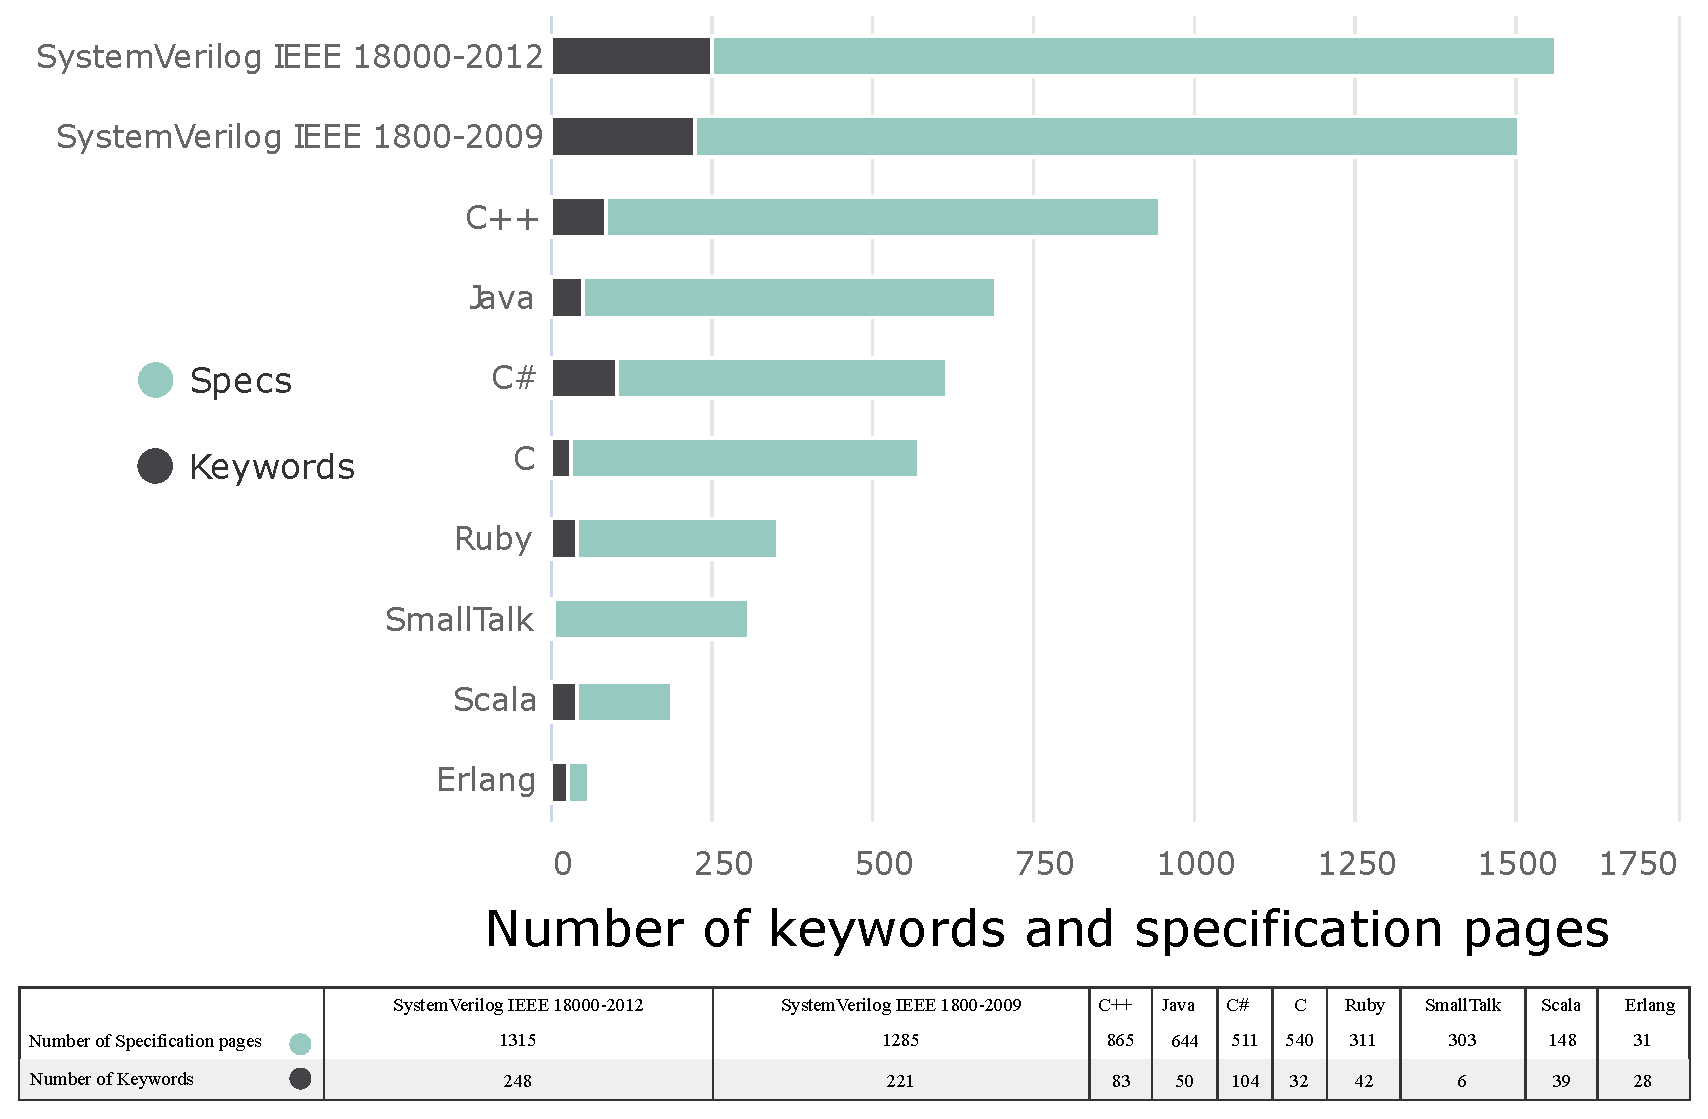
\includegraphics[width=\linewidth]{pictures/Complexity_of_a_language.eps}
\caption{Language complexity \cite{presentation:cerncocotb}.}
\label{fig:languagecomplexity}
\end{figure}

\section{Organization}
This document presents the following structure:
\begin{description}
\item[Chapter \ref{stateofart}] : provides some background regarding hardware
  description languages, from the traditional to the newer ones. Morover, it
  gives a general look at the technology that are currently used for hardware
  verification.
\item[Chapter \ref{functionalverification}] : introduces the concept of
  functional verification and it compares this new type of verification with the
  traditional methodology.
\item[Chapter \ref{constraintrandom}] : takes a closer look at one of the
  branches of functional verification called Constrained Random Verification. In
  this chapter, the theory behind CRV and Constraint Satisfaction Problems is
  introduced together with standard solution algorithms to solve these problems.
\item[Chapter \ref{fcsp}] : presents F-CSP, a completely new library entirely
  developed in Scala that integrated Constraint Random Verification into Chisel
  but was then abandoned because of its lousy performance and low
  maintainability.
\item[Chapter \ref{chiselcrv}] : presents Chisel-CRV, a new library for
  Constraint Random Verification, born after F-CSP and based on the JaCoP Java
  library for constraint programming.
\item[Chapter \ref{verificationalu}] : combines the technique described in
  chapters 5 and 6 and the Chisel-CRV library together with the chiselverify one
  to functionally verify the Leros ALU.
\item[Chapter \ref{conclusion}] : conclusion.
\end{description}

\section{Remarks about Verification and Testing}
Before reading the present document, it is necessary to clarify the distinction
between verification and testing. These two terms in the literature are often
presented with a different meaning. Generally speaking, in the hardware world,
testing is often a synonym for the actual physical action of testing a device
after its fabrication. In the same domain, verification refers to the process of
ensuring that the model behaves according to the specifications before it is
produced. On the other hand, in the software world, the two terms have a more
subtle difference, where verification refers to validating the software
architecture specification, and testing refers to the software's actual
validation. While these two terms have a separate meaning for these two distinct
worlds, the separation becomes more blurred when the hardware description
language used to generate the hardware models lives in a software domain. For
this reason, the author decided strictly to avoid dogmatizing either of the two
terms and use them interchangeably throughout the document with the meaning of
verifying the device functionality before it is produced.
